\chapter{Other low-energy physics with P-type point contact detectors}

		
	\section{Signal from Heavy Axions}
	\label{sec:CalcLimitsOnHeavyAxions}		
		
		\begin{figure}
			\centering
			%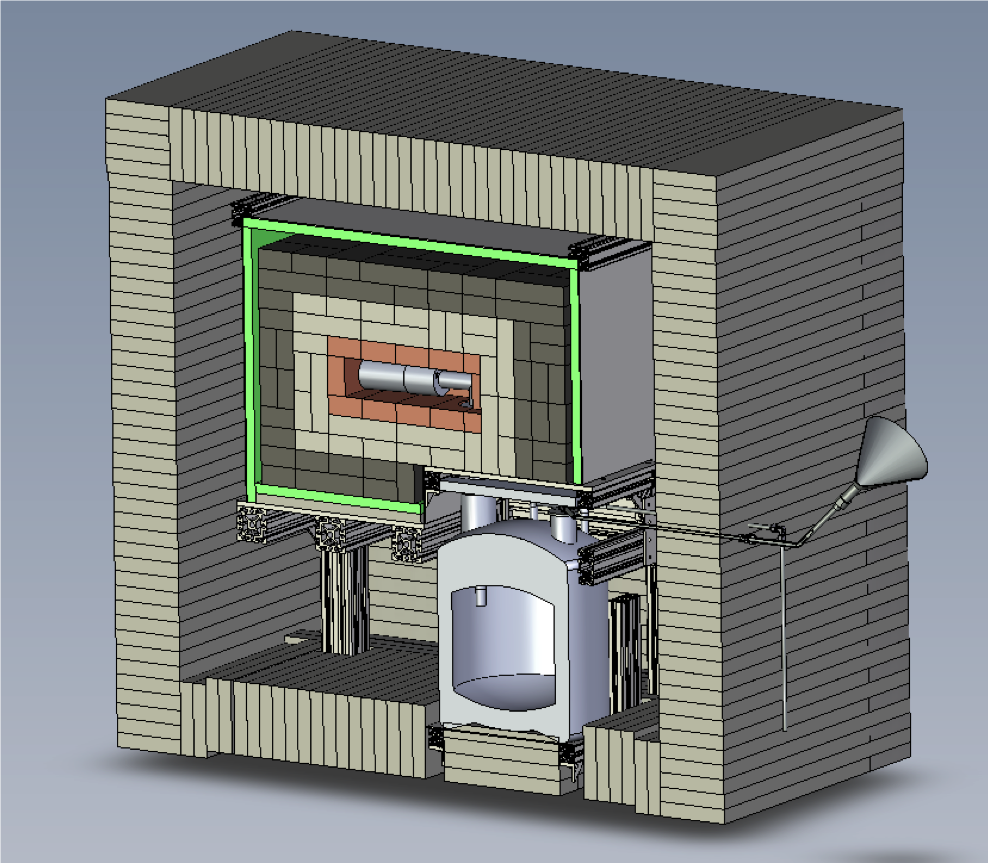
\includegraphics[width=0.9\textwidth]{PPC2DesignSchematicAll}
			\caption{Possible Heavy Axion Dark Matter signal.}
			\label{fig:HeavyAxionSignal}
		\end{figure}
				
	\subsection{Generic oscillation signal}
	\label{sec:CalcLimitsOnGenericalOscillationSignal}		
		
		\begin{figure}
			\centering
			%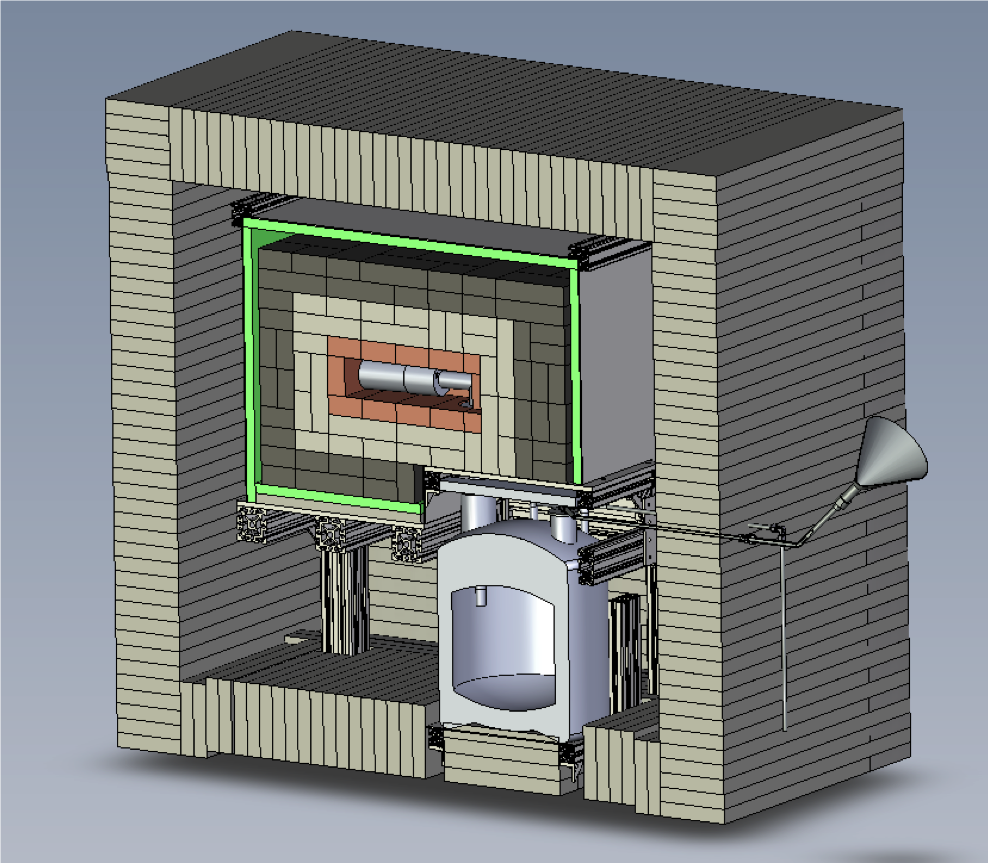
\includegraphics[width=0.9\textwidth]{PPC2DesignSchematicAll}
			\caption{A generic oscillation signal with an amplitude of.}
			\label{fig:GenericOscillationSignal}
		\end{figure}
		
							
	\section{Sensitivity of the \MJ~\minmod~to a Dark Matter signal}
		\subsection{Low-energy background model}
		\label{sec:MJLowEnergyBackgroundModel}
		\subsection{WIMPs}
		\label{sec:MJSensitivityToWIMP}
		
			\begin{figure}
				\centering
				%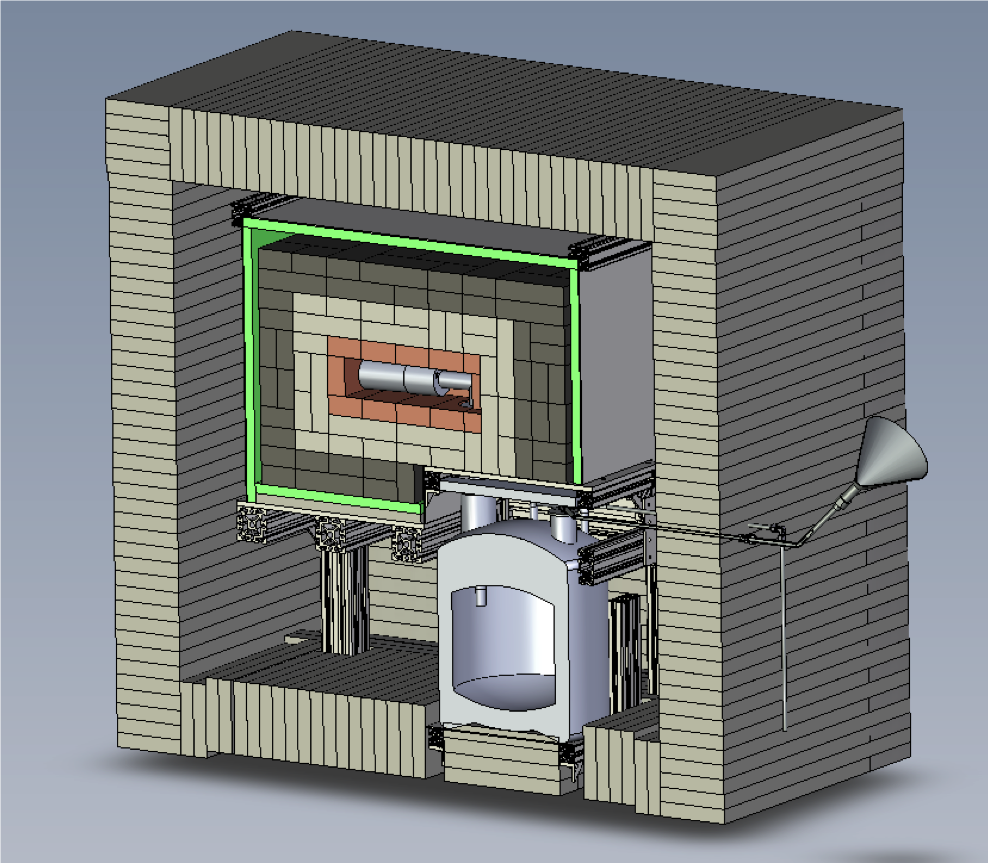
\includegraphics[width=0.9\textwidth]{PPC2DesignSchematicAll}
				\caption{\MJ~\minmod~sensitivity to a WIMP signal.}
				\label{fig:MJSensitivityToWIMP}
			\end{figure}		
		\subsection{Heavy Axions}
		\label{sec:MJSensitivityToAxions}
		
			\begin{figure}
				\centering
				%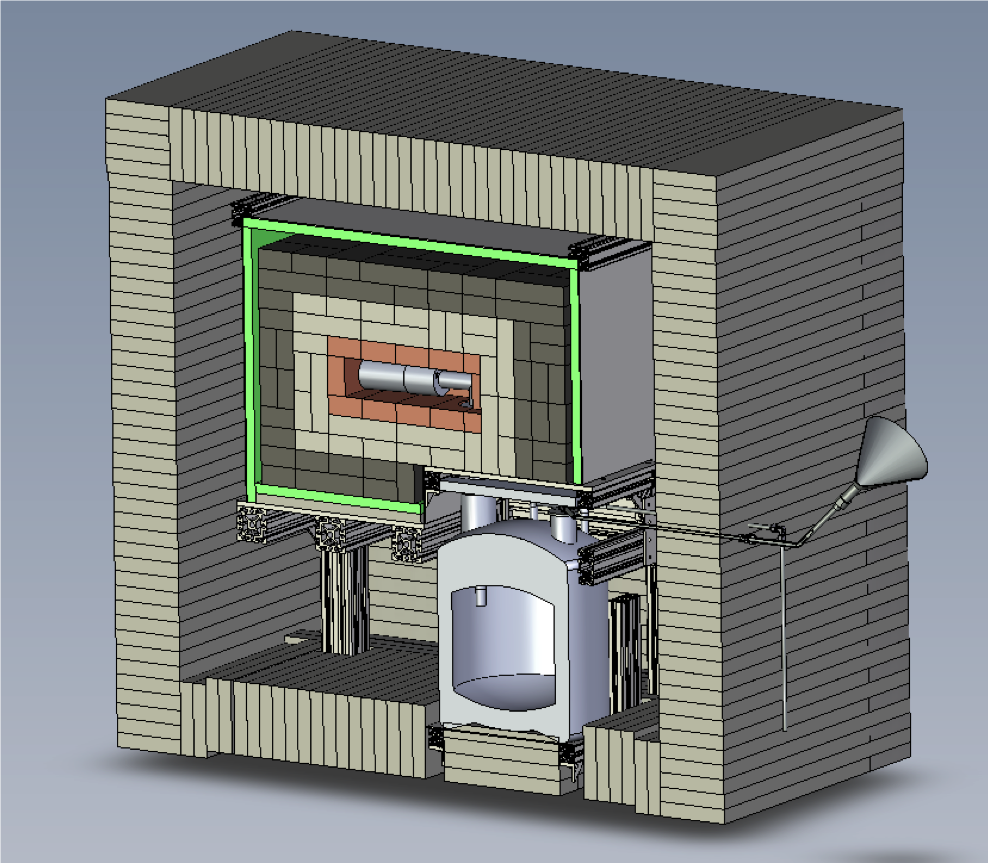
\includegraphics[width=0.9\textwidth]{PPC2DesignSchematicAll}
				\caption{\MJ~\minmod~sensitivity to a Heavy Axion signal.}
				\label{fig:MJSensitivityToHeavyAxions}
			\end{figure}		
		\subsection{Generic Oscillation Signal}
		\label{sec:MJSensitivityToGenOsc}
		
			\begin{figure}
				\centering
				%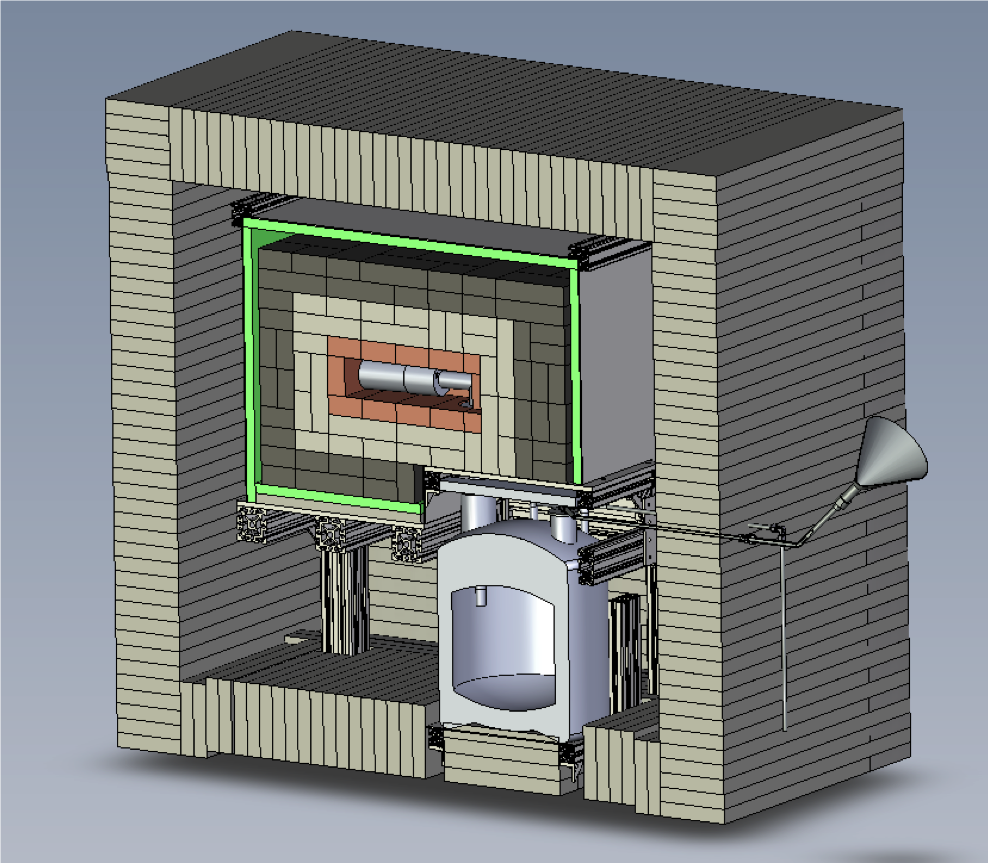
\includegraphics[width=0.9\textwidth]{PPC2DesignSchematicAll}
				\caption{\MJ~\minmod~sensitivity to a generic oscillation signal.}
				\label{fig:MJSensitivityToGenOscSignal}
			\end{figure}		
	
	%\subsection{Heavy Axions}
	%\label{sec:LimitsToAxions}
	%	\begin{figure}
	%		\centering
	%		%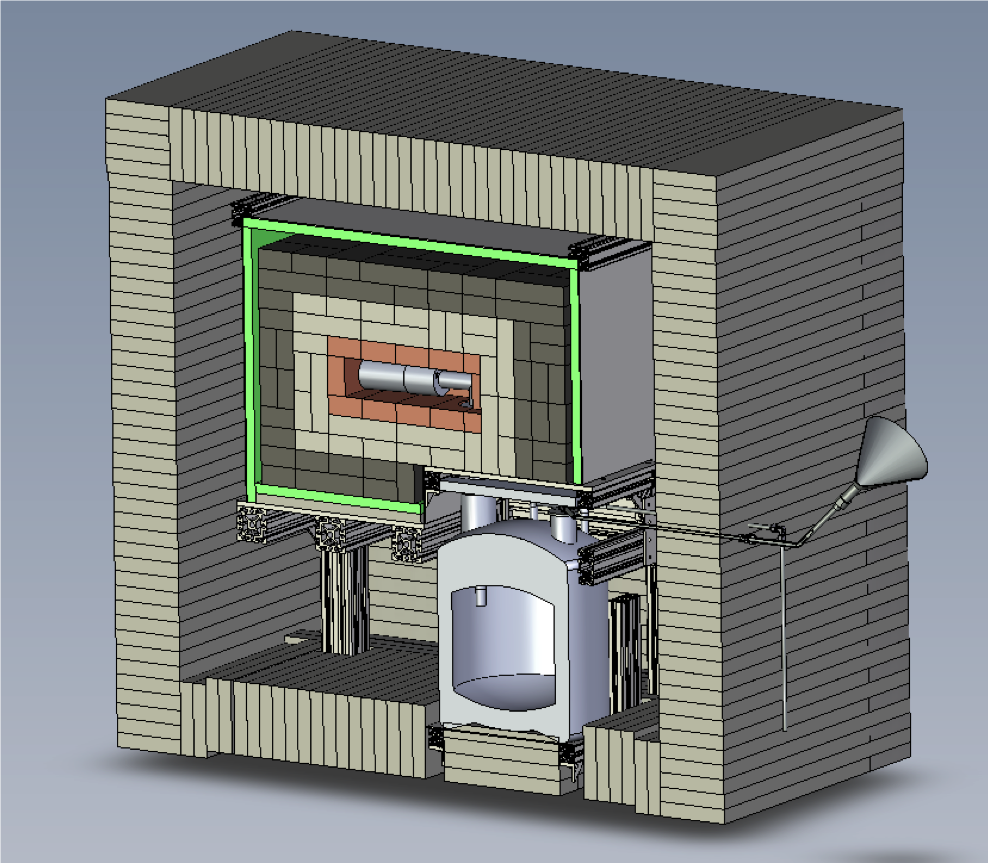
\includegraphics[width=0.9\textwidth]{PPC2DesignSchematicAll}
	%		\caption{Limits on Heavy Axions.}
	%		\label{fig:BeGeLimitsOnHeavyAxions}
	%	\end{figure}				
